\documentclass[aspectratio=169]{beamer}
\beamertemplatenavigationsymbolsempty
\usepackage{qrcode}

\usepackage{parskip, setspace}
\setstretch{1.5}

\usepackage{biblatex}
\addbibresource{bib.bib}
% math formatting
\usepackage{amsmath, amsfonts, braket}
% \numberwithin{equation}{section}
% rich text
\usepackage{graphicx, caption}
\usepackage{hyperref}
\usepackage{xcolor}
\hypersetup{
    colorlinks=false,
    linkcolor=black,  
    urlcolor=blue,
    citecolor=blue,
    pdftitle={Chapman SOURCE 2024},
    pdfpagemode=FullScreen,
}

\usepackage[ruled,linesnumbered,lined,boxed,commentsnumbered]{algorithm2e}

\usetheme{Madrid}
\title[Analog Particles with HPC]{Modelling Particle Production in Analog Expanding Universes with High-Performance Computing}
% \subtitle{}

\author[Chapman, Nathan]{Nathan Chapman}

\institute[CWU]
{
  Department of Computer Science \\
  Department of Physics \\
  Central Washington University
%   \and
%   \inst{2}%
%   Faculty of Chemistry\\
%   Very Famous University
}

\date[SOURCE 2024]{CWU SOURCE 2024}

\logo{
\includegraphics[height=0.5cm]{images/cwu_logo.png}}

\begin{document}

\frame{\titlepage}
% \begin{frame}
%     \frametitle{Table of Contents}

%     \tableofcontents

% \end{frame}

\section{Introduction}
\subsection{}
\begin{frame}
    \frametitle{Introduction - Analog Universes}

    \begin{columns}
        \begin{column}{0.5\textwidth}
            \begin{enumerate}
                \item <1->Inflation created particles
                \item <2->Cannot directly observe these particles
                \item <3->Theory suggests ultra-cold quantum gases behave similarily
                \item <4->Can make gas in the lab $\implies$ can \emph{effectively} observe inflation particles
                \item <5->Lab based system = ``analog universe''
            \end{enumerate}
        \end{column}
        \begin{column}{0.5\textwidth}
            \begin{figure}
                \centering
                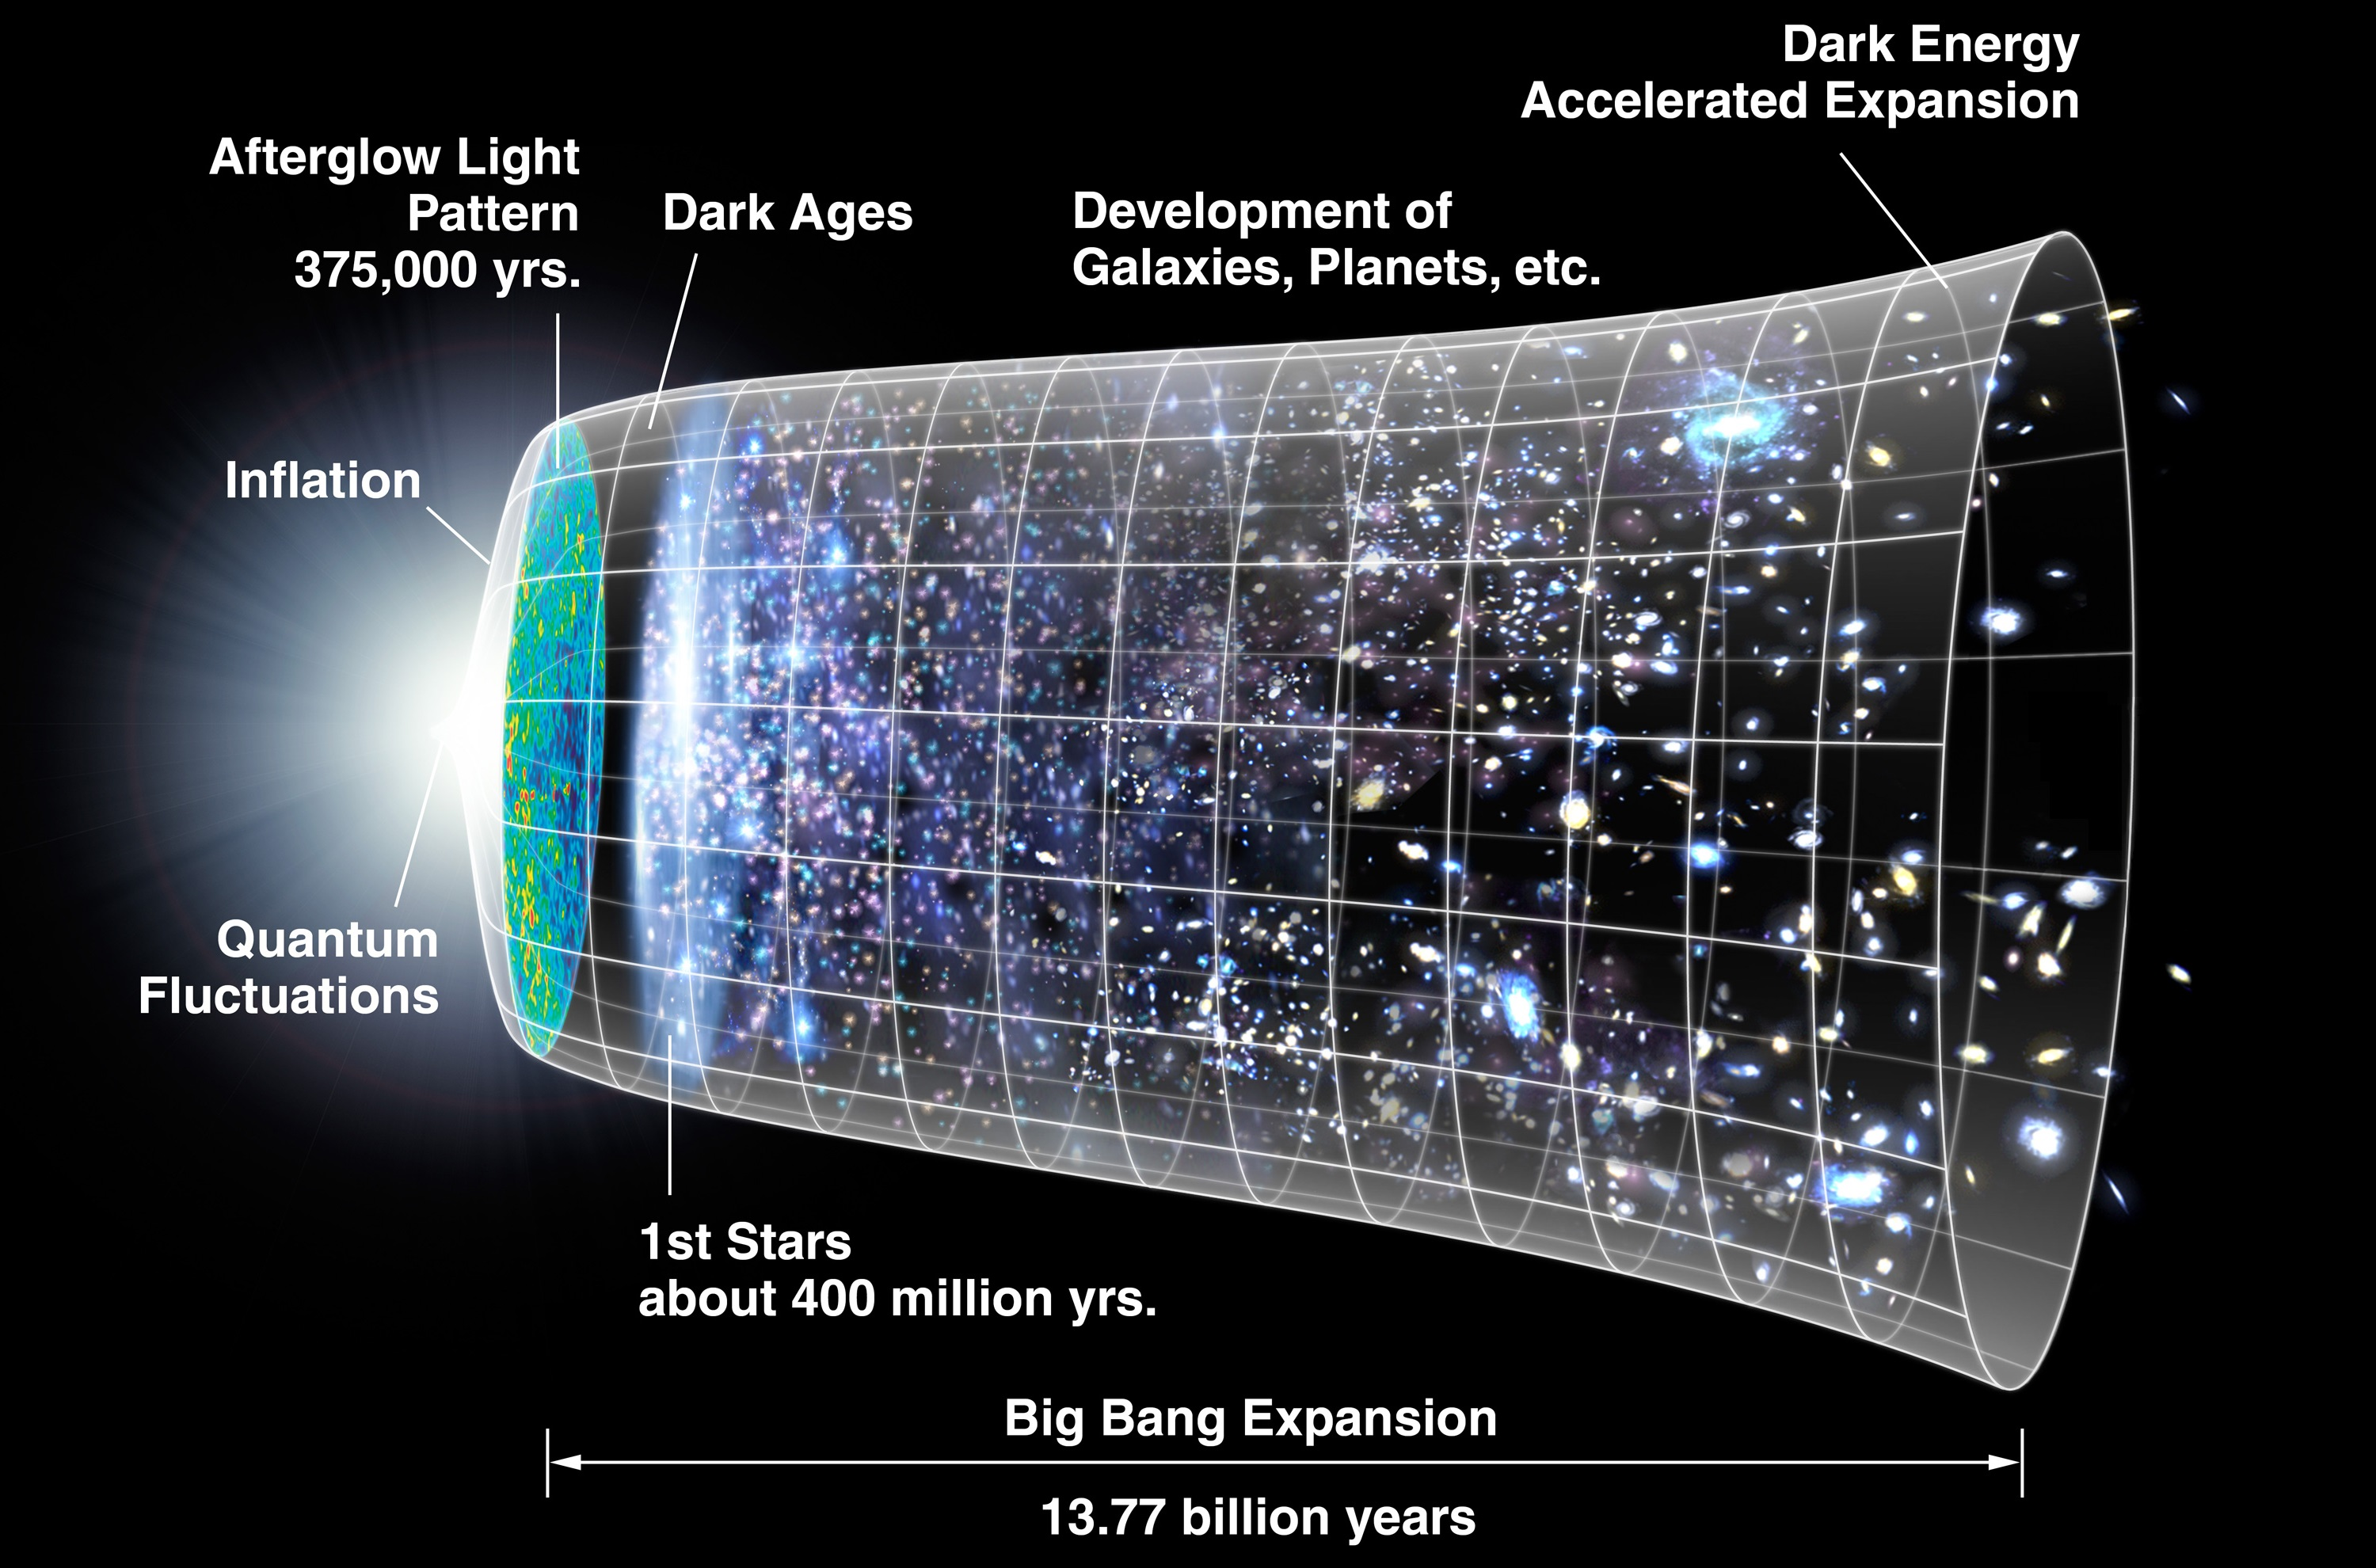
\includegraphics[width=\textwidth]{images/CMB_Timeline300_no_WMAP.jpg}
                \caption{History of the universe highlighting period of rapid expansion (\href{https://upload.wikimedia.org/wikipedia/commons/6/6f/CMB_Timeline300_no_WMAP.jpg}{Source})}
            \end{figure}
        \end{column}
    \end{columns}
\end{frame}

\begin{frame}
    \frametitle{Introduction - The Story So Far}

    \begin{columns}
        \begin{column}{0.5\textwidth}
            \begin{itemize}
                \item <1->Many investigations into analog universes
                \item <2->Few into exact analogs
                \item <3->Fewer into computational simulation
                \item <4->Even fewer using high-performance computing
            \end{itemize}
        \end{column}
        \begin{column}{0.5\textwidth}
            \begin{figure}
                \centering
                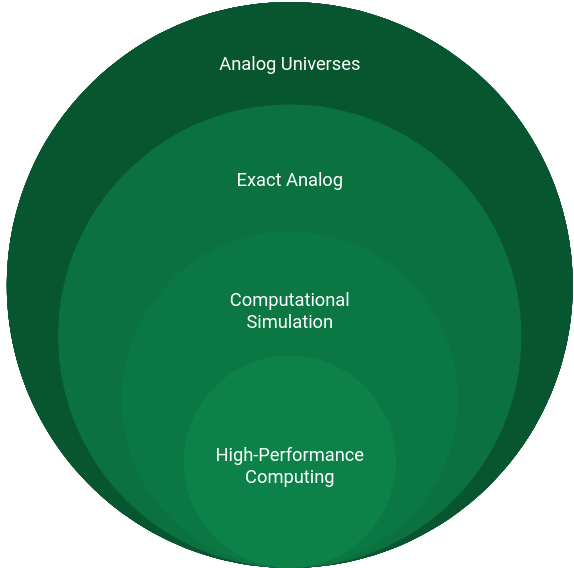
\includegraphics[width=0.7\textwidth]{images/subsets.png}
                \caption{Subsets of increasingly specific literature}
            \end{figure}
        \end{column}
    \end{columns}

\end{frame}

\section{Theory}
\subsection{Speed \& Expansion}
\begin{frame}
    \frametitle{Methods - Speed \& Expansion}
    \begin{columns}
        \begin{column}{0.5\textwidth}
            \begin{itemize}
                \item <1->Speed of sound in quantum gas =\\ Speed of light in analog universe
                \item <2->Speed decrease \& static volume $\iff$ constant speed \& expanding volume
                \item <3->Example: $t = d/v$
                \begin{itemize}
                    \item Distance to grocery store doubles $\implies$ travel time doubles
                    \item Speed to the grocery store halves $\implies$ travel time doubles
                \end{itemize}
            \end{itemize}
        \end{column}
        \begin{column}{0.5\textwidth}
            \vspace{0.3in}
            \begin{figure}
                \centering
                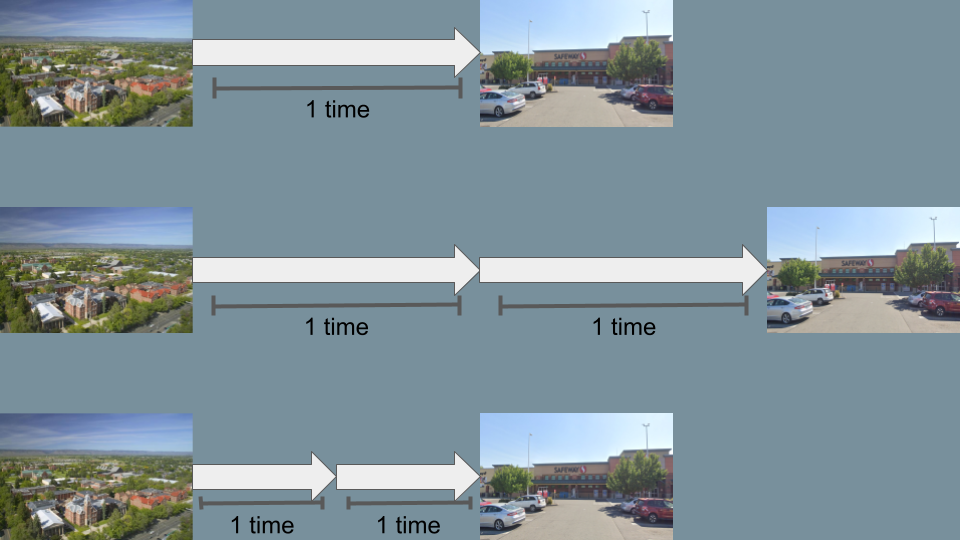
\includegraphics[width=\textwidth]{images/Untitled presentation.png}
                \caption{Travel time can be doubled by either doubling distance or halving speed}
            \end{figure}
        \end{column}
    \end{columns}
\end{frame}

\subsection{Mathematical Model}
\begin{frame}
    \frametitle{Methods - The Field Equation}
    \setstretch{1.25}
    \begin{itemize}
        \item One equation describes both ultra-cold quantum gases and inflation particles
        \item One equation for each $k < k_c$ % and $\hbar^2 k_c^2 / 2 m = U n_0$
        \item Universe expansion starts and stops at finite times % $\implies \eta_i \leq \eta \leq \eta_f$
    \end{itemize}
    
    \begin{exampleblock}{\centering The Field Equation}
        \begin{subequations}
            \begin{equation*}
                \underbrace{\partial_\eta^2 \widetilde{\theta}_\mathbf{k} - c_0^2 k^2 \widetilde{\theta}_\mathbf{k}}_\text{Wave} - \underbrace{\frac{1}{2} \frac{\dot{a}(\eta)}{a(\eta)} \partial_\eta \widetilde{\theta}_\mathbf{k}}_\text{Damping} = 0
            \end{equation*}
            \vspace{-0.2in}
            \begin{equation*}
                \widetilde{\theta}_\mathbf{k}(0) = \widetilde{\theta}_{\mathbf{k}0} \quad \partial_\eta \widetilde{\theta}_\mathbf{k}(0) = -U_0 n_{\mathbf{k}0} / \hbar
            \end{equation*}
        \end{subequations}
    \end{exampleblock}
\end{frame}

\subsection{Computational Model}
\begin{frame}
    \frametitle{Methods - Solving The Field Equation}
    \begin{columns}
        \begin{column}{0.5\textwidth}
            \begin{itemize}
                \item <1->Need to try to conserve energy
                \item <2->Use \emph{symplectic integrator}
                \item <3->Use new momentum to calculate position
                \item <4->More complex but more stable
            \end{itemize}
        \end{column}
        \begin{column}{0.5\textwidth}
            \begin{figure}
                \centering
                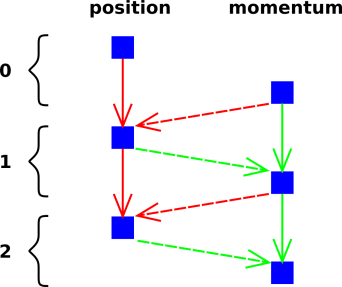
\includegraphics[width=0.8\textwidth]{images/integrator-symplectic-stagger.png}
                \caption{Symplectic integrator example: Velocity Verlet \href{https://www.av8n.com/physics/symplectic-integrator.htm}{(Source)}}
            \end{figure}
        \end{column}
    \end{columns}

\end{frame}

\begin{frame}
    \frametitle{Methods - High-Performance Computing}

    \begin{columns}
        \column{0.6\textwidth}
            \begin{itemize}
                \item <1->Equation for each $k < k_c$
                \item <2->Many equations to solve
                \item <3->Solve at the same time with multiple GPUs
                \item <4->Use CWU's ``Turing'' supercomputer
                \item <4->4x4 NVIDA P100 GPUs \\- Each 83\% performance of modern RTX 3060
                % \item 180 GBps GPU-GPU bandwidth
                % \item 80 GBps (NVLink) GPU-CPU bandwidth
            \end{itemize}
        \column{0.4\textwidth}
            \begin{figure}[h]
                \centering
                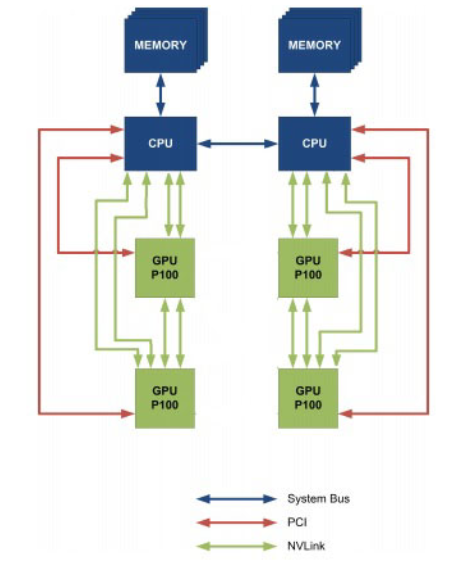
\includegraphics[height=0.65\textheight]{images/NVLink.png}
                \caption{CPU to GPU and GPU to GPU interconnect using NVLink}
            \end{figure}
    \end{columns}

\end{frame}
\section{Analytic Results}
\subsection{Final Time Distribution}
\begin{frame}
    \frametitle{Analytic Results - Simple Expansion}

    \begin{columns}
        \begin{column}{.5\textwidth}
            % \vspace{-0.5in}
            \begin{itemize}
                \item <1->Simple expansion: $a(t) = e^{-t/t_s}$
                \item <2->Use Mathematica for analytic results
                \item <3->Population distribution highly depends on length of expansion
                \item <4->Population is relatively high for low $k$
                \item <5->Population drops off quickly with $k$
            \end{itemize}
        \end{column}
        \begin{column}{.5\textwidth}
            \vspace{0.5in}
            \begin{figure}[h]
                \centering
                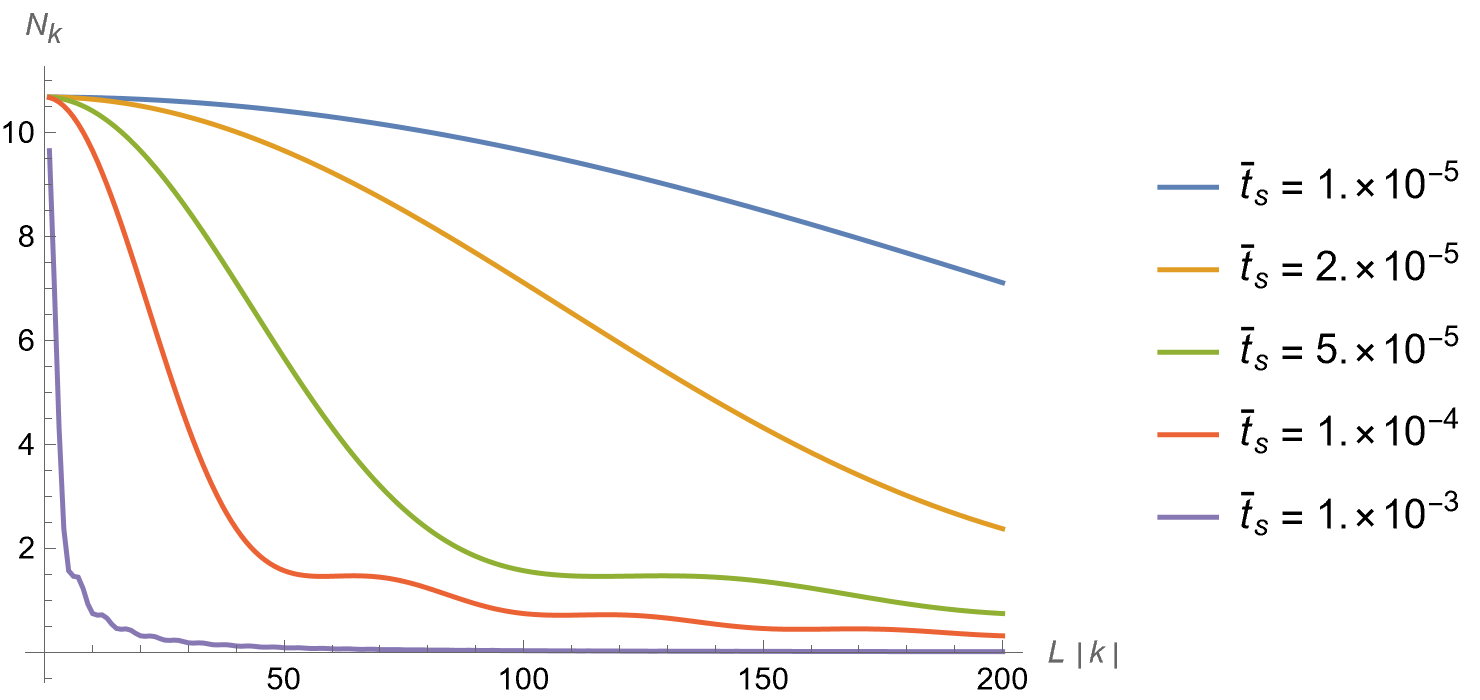
\includegraphics[width=\textwidth]{images/fig2.png}
                \caption{The momentum distribution when the universe stops expanding for multiple effective \\ rates of expansion}
                \label{fig:finalTime}
            \end{figure}
        \end{column}
    \end{columns}
\end{frame}

\subsection{All Time Distribution}
\begin{frame}
    \frametitle{Analytic Results - Simple Expansion}

    \begin{figure}[h]
        \centering
        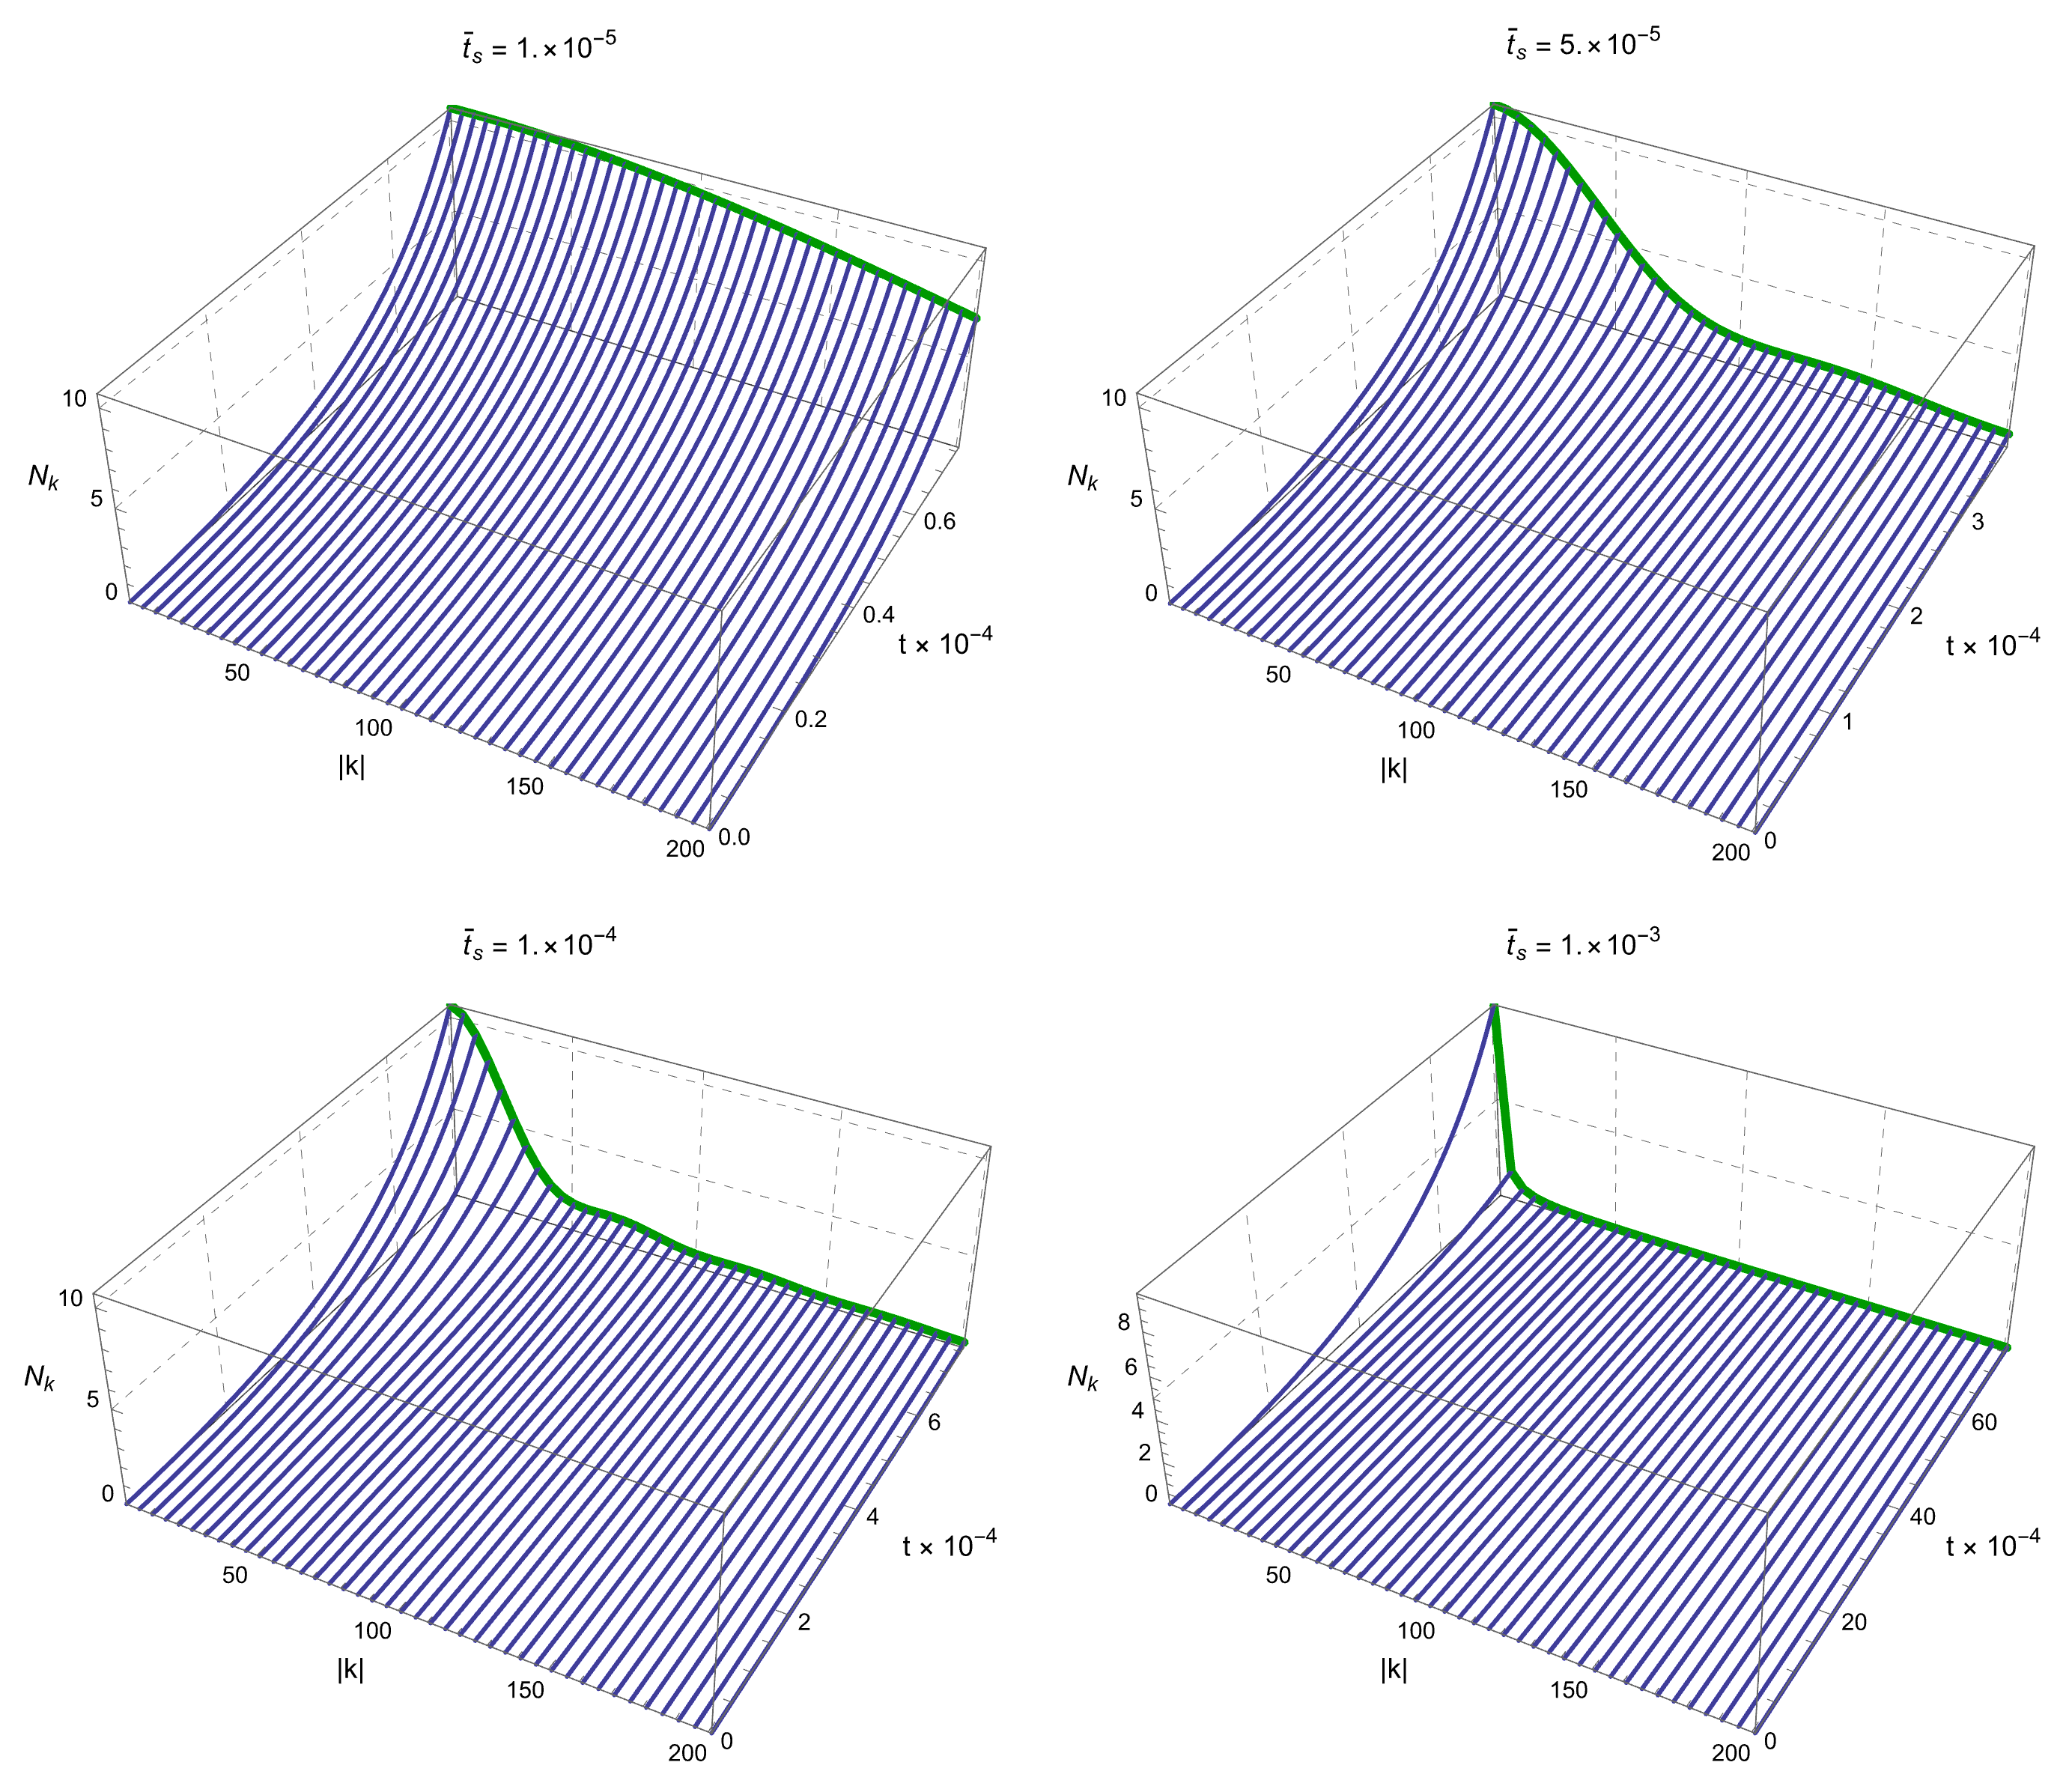
\includegraphics[height=0.74\textheight]{images/Analytic_Fig_4.png}
        \caption{Momentum distribution throughout the expansion}
        \label{fig:allTime}
    \end{figure}

\end{frame}

\begin{frame}
    \frametitle{Conclusion}
    \setstretch{1.25}
    \begin{itemize}
        \item <1->An inflating universe looks the same as an ultra-cold quantum gas with a decreasing speed of sound
        \item <2->Theory suggests inflation particles behave the same as ultra-cold quantum gases in the lab
        \item <3->There are many equations that need to be solved with special methods to conserve energy
        \item <4->Use high-performance techniques and hardware for reasonable execution time
        \item <5->Expect the distribution of momenta to depend on the length of the expansion
        \item <6->Expect the population to be high for low $k$ and drop off quickly
    \end{itemize}
\end{frame}

\begin{frame}
    \frametitle{Acknowledgements}

    \begin{itemize}
        \item Dr. Andy Piacsek (CWU, Physics)
        \item Dr. Szilard VAJDA (CWU, Computer Science)
        \item Dr. Micheal Braunstein (CWU, Physics)
        \item Dr. Brandon Peden (WWU, Physics \& Astronomy)
    \end{itemize}

\end{frame}

\begin{frame}{Thank you \& Code source}
    \begin{columns}[onlytextwidth]
        \begin{column}{.5\textwidth}
            Thank you for your attention.
            \vspace*{0.1\textheight} \\
            The code for this project is available at:
            \begin{itemize}
                \item GitHub (QR code): \url{github.com/nondairyneutrino/thesis}
                \item My website: \url{nathanwchapman.com}
            \end{itemize}
        \end{column}
        \begin{column}{.5\textwidth}
            \centering
            \qrcode[height=0.67\textheight]{https://github.com/nondairyneutrino/thesis}
        \end{column}
    \end{columns}
    \end{frame}

% \begin{frame}[allowframebreaks]
%     \frametitle{\bibname}
%     \nocite{*}
%     \printbibliography
% \end{frame}

\end{document}